\documentclass[12pt,a4paper]{article}

\usepackage{tikz}
\usetikzlibrary{automata, positioning, arrows}

\begin{document}
\title{Automata}
\maketitle

\section{Introduction}

\begin{equation}
    \sum = \{0,1\}
\end{equation}

\begin{equation}
    L(M_1) = \{\omega \in \sum^\ast | \omega .endsWith(00)\}
\end{equation}
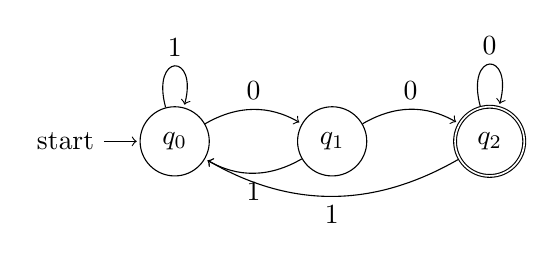
\begin{tikzpicture}[shorten >=1pt,node distance=2cm,on grid,auto] 
   \node[state, initial] (q_0) {$q_0$};
   \node[state, right=of q_0] (q_1) {$q_1$};
   \node[state, accepting, right=of q_1] (q_2) {$q_2$};
   \path[->] 
    (q_0) edge [bend left, above] node {0} (q_1)
          edge [loop above] node {1} ()
    (q_1) edge [bend left, above] node {0} (q_2)
          edge [bend left, below] node {1} (q_0)
    (q_2) edge [loop above] node {0} ()
          edge [bend left, below] node {1} (q_0);
\end{tikzpicture}

\begin{equation}
    L(M_2) = \{\omega \in \sum^\ast | \omega .contains(000)\}
\end{equation}
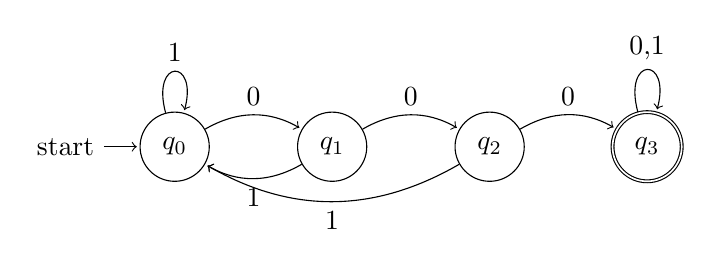
\begin{tikzpicture}[shorten >=1pt,node distance=2cm,on grid,auto] 
    \node[state, initial] (q_0) {$q_0$};
    \node[state, right=of q_0] (q_1) {$q_1$};
    \node[state, right=of q_1] (q_2) {$q_2$};
    \node[state, accepting, right=of q_2] (q_3) {$q_3$};
    \path[->]
        (q_0) edge [bend left, above] node {0} (q_1)
            edge [loop above] node {1} ()
        (q_1) edge [bend left, above] node {0} (q_2)
            edge [bend left, below] node {1} (q_0)
        (q_2) edge [bend left, above] node {0} (q_3)
            edge [bend left, below] node {1} (q_0)
        (q_3) edge [loop above] node {0,1} ();
 \end{tikzpicture}

\end{document}
